\documentclass[a4paper,1pt,oneside]{article}
\usepackage{graphicx}
\usepackage{xcolor}
\usepackage{titlesec}
\usepackage{indentfirst}
\usepackage{setspace}
\usepackage{enumitem}
\usepackage[utf8]{inputenc}

\titleformat{\section}{\Large\bfseries}{\thesection}{1em}{}[{\titlerule[0.8pt]}]

\title{\textsc{Assignment - 1\\Web Designing}}
\author{Abhay Shanker Pathak}
\date{March 2020}

\begin{document}

\maketitle
\setlength{\parindent}{1cm}

\renewcommand{\abstractname}{About}
\begin{abstract}
	\centering
	This assignment contatins screenshots of solved examples\\
	for \textbf{Cascading Sytle Sheet}
\end{abstract}

\pagenumbering{roman}
\tableofcontents
\listoftables
\listoffigures

\clearpage

\pagenumbering{arabic}

\section{Introduction}

\begin{itemize}
	\item \textbf{Sytle Sheet} is a document that contain style information about one or more documents written in markup languages.
	\item A style sheet is composed of a set of style rules written in specified format.
	\item \textbf{Cascading Sytle Sheet(CSS)} is style sheet language that specifies how to incorporate style information in a style sheet. The term cascading indicates that several style sheets can be blended to preset a document on the browser's screen.
\end{itemize}

\section{Adding CSS}

\begin{itemize}
	\item There are four ways to specify style information in a document
		\begin{itemize}
			\item External Sytle Sheet
			\item Embedded Style Sheet
			\item Imported Style Sheet
			\item Inline Style Sheet
		\end{itemize}
\end{itemize}

\subsection{External Style Sheet}

\begin{itemize}
	\item In this case style information is written in a separate file and referenced from an HTML document.
	\item An external style sheet is useful when the same style is applied on different documents.
	\item The external style sheet is specified using the HTML \textless link \textgreater tag.
	\item \textless link rel = ``stylesheet'' type = ``text/css'' href = ``mystyle.css''/ \textgreater
\end{itemize}

Below is the example code for \textbf{External Style Sheet}

\begin{figure}[hbt!]
	\centering
	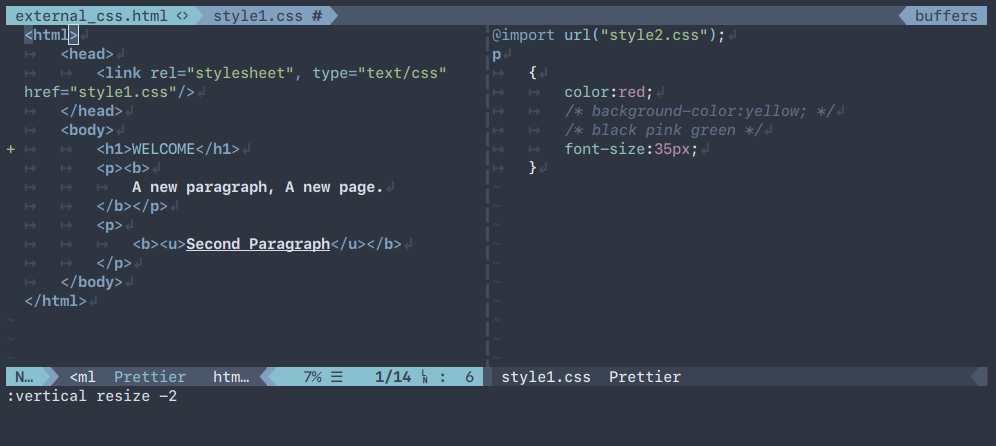
\includegraphics[width=1\textwidth]{images/2020-03-23-224542_996x446_scrot.png}
	\caption{Showing external style sheet with vsplit}
\end{figure}

\subsection{Embedded Style Sheet}

\begin{itemize}
	\item In this method style information is placed under the style tag in the head section of an HTML page.
\end{itemize}

See the example to learn more

\begin{figure}[hbt!]
	\centering
	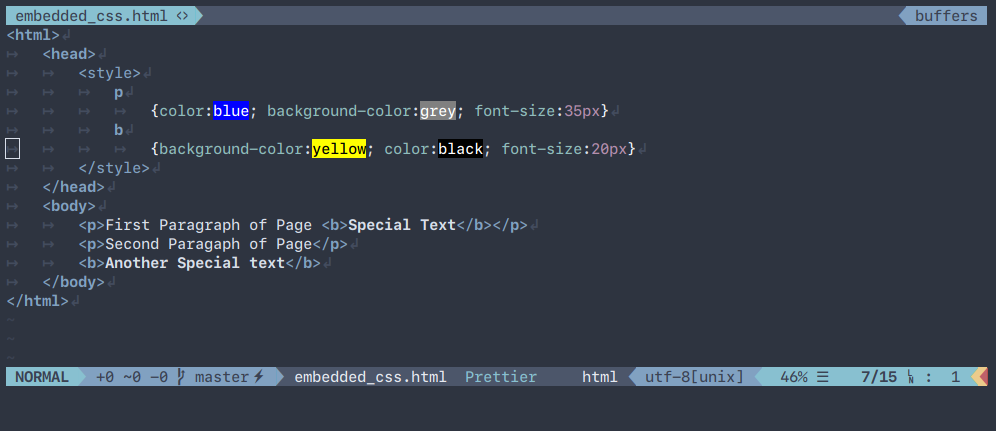
\includegraphics[width=1\textwidth]{images/2020-03-23-224635_996x431_scrot.png}
	\caption{Example of Embedded Style Sheet}
\end{figure}

\subsection{Imported Style Sheet}

\begin{itemize}
	\item Another way of importing stylesheet is to use \textcolor{blue}{\textbf{@import}} statement. It allows importing style sheet from another style sheet.
\end{itemize}

Here's the example below of imported style sheet

\begin{figure}[hbt!]
	\centering
	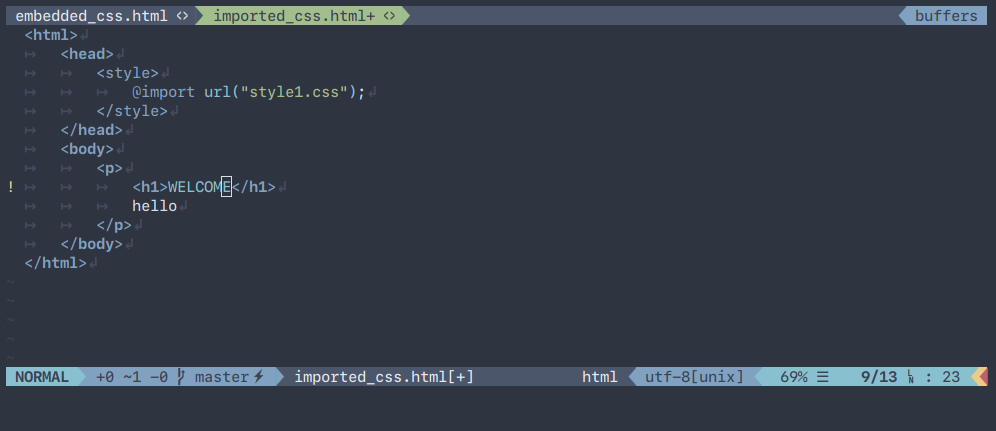
\includegraphics[width=1\textwidth]{images/2020-03-23-224759_996x431_scrot.png}
	\caption{exaple showing imported style sheet}
\end{figure}

\subsection{Inline Style Sheet}

\begin{itemize}
	\item In this case style information is incorporated directly into the HTML tags.
	\item \textless p style = ``color:red'' \textgreater Hello World </p>
\end{itemize}

See the example of inline style sheet

\begin{figure}[hbt!]
	\centering
	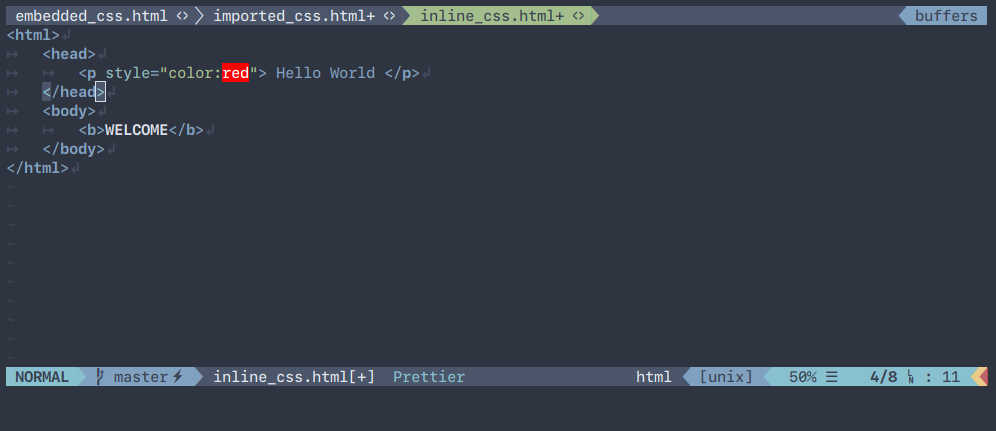
\includegraphics[width=1\textwidth]{images/2020-03-23-225058_996x431_scrot.png}
	\caption{exaple showing inline style sheet}
\end{figure}

\section{Selectors In CSS}

\noindent Selector determines on which rules are to be applied. The elements selected by the selector are called \textcolor{orange}{\textbf{subjects of selectors}}.

Here are few types of selectors:

\subsubsection{Simple Selector}

Element is selected by it's name.

\begin{figure}[hbt!]
	\centering
	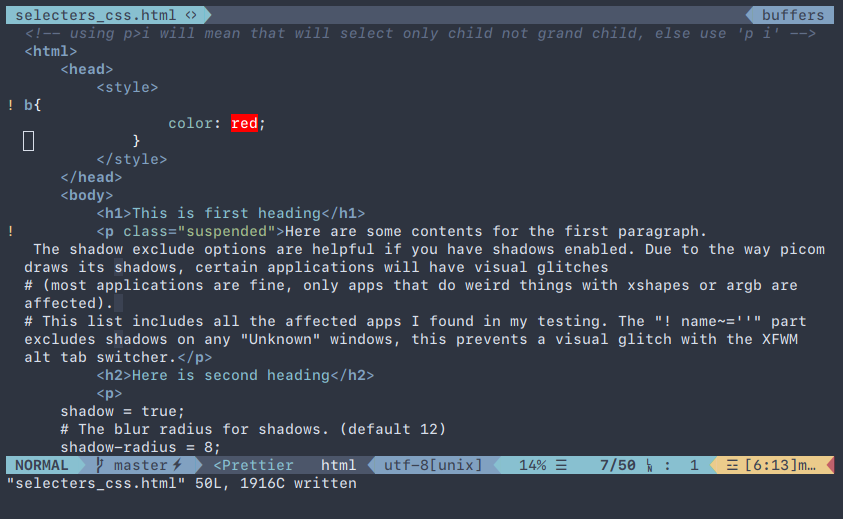
\includegraphics[width=0.7\textwidth]{images/2020-03-24-002817_843x519_scrot.png}
	\caption{an example of simple selector}
\end{figure}

\subsubsection{Grouping:}
Selectors having common declaration are grouped into a comman separated list

here's the screenshot

\begin{figure}[hbt!]
	\centering
	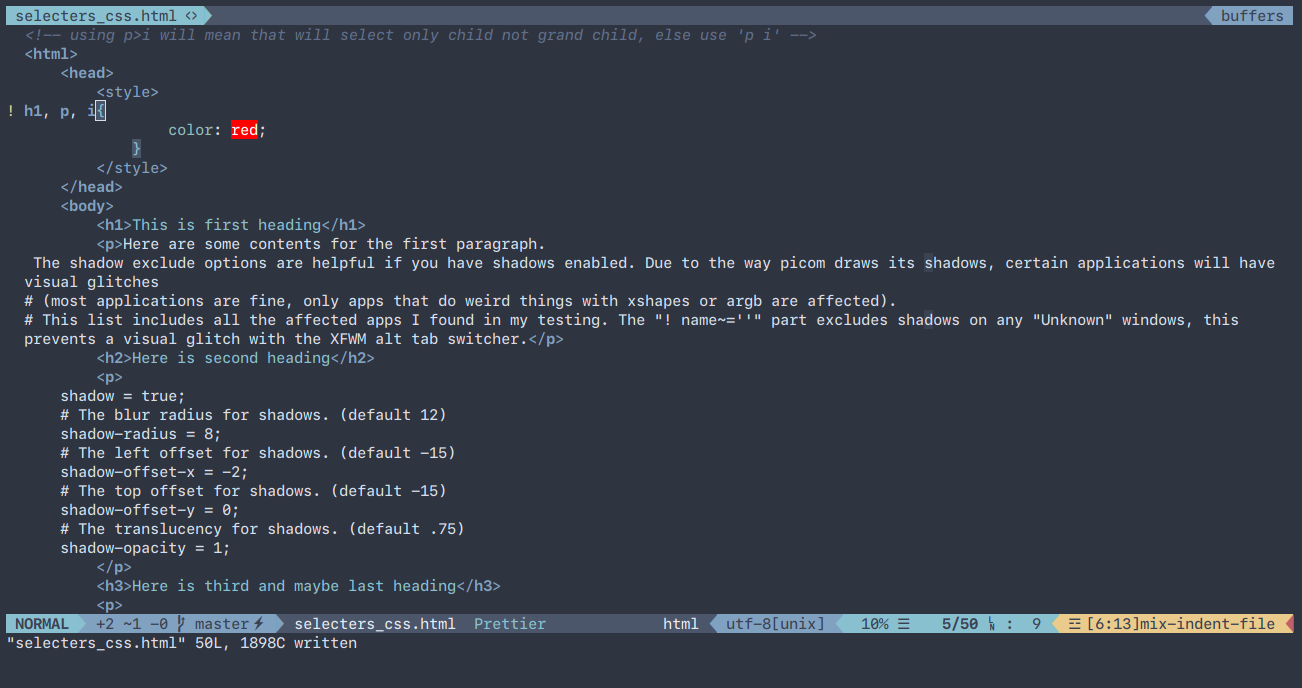
\includegraphics[width=1\textwidth]{images/2020-03-23-225413_1302x688_scrot.png}
	\caption{example of grouping}
\end{figure}

\subsubsection{Universal selectors:}
CSS has special type of selector * which matches with every single element in teh document

Showed in following screenshot

\begin{figure}[hbt!]
	\centering
	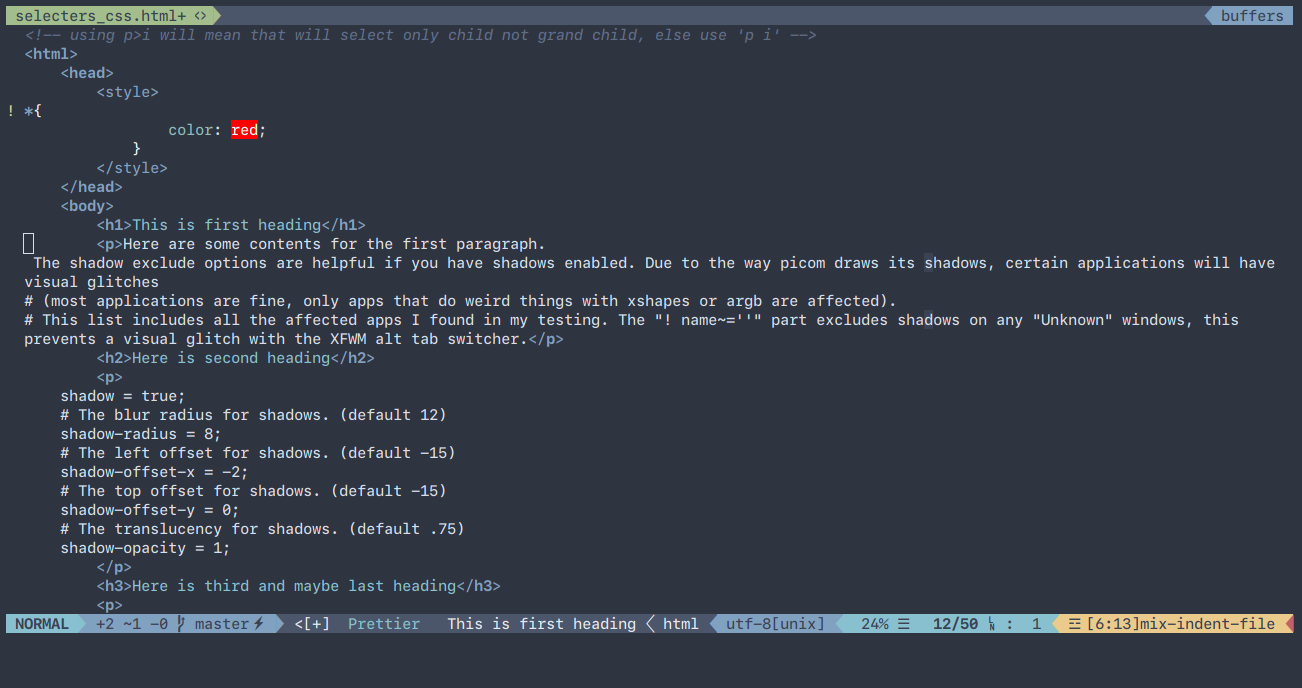
\includegraphics[width=1\textwidth]{images/2020-03-23-225436_1302x688_scrot.png}
	\caption{example of universal selector}
\end{figure}

\subsubsection{Descendent Selector}
Descendent selectors, allow us to determines the elements depending upon the their hierarchical relationship.

For example:

\begin{figure}[hbt!]
	\centering
	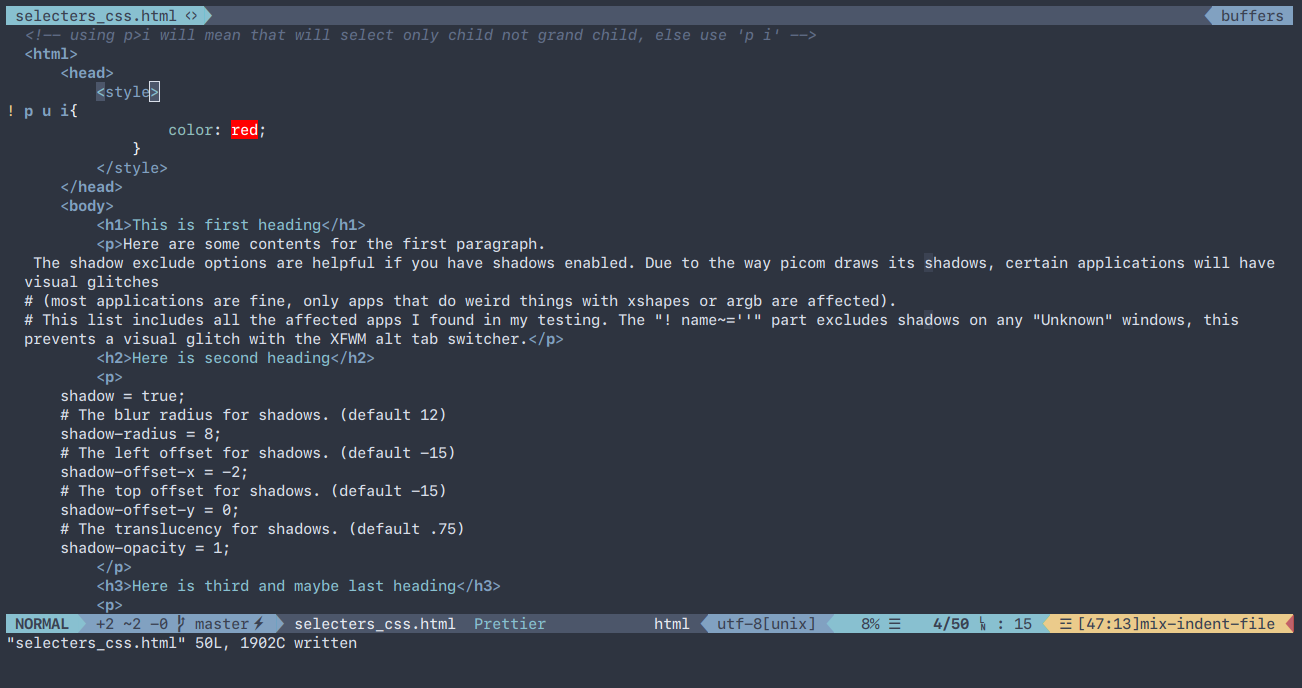
\includegraphics[width=1\textwidth]{images/2020-03-23-225534_1302x688_scrot.png}
	\caption{exaple showing descendant selectors}
\end{figure}

\subsubsection{Child Selector}

Child selector select elements that are immediate children of a specified element. The combinator used for child selector is ``)''.

For example:

\begin{figure}[hbt!]
	\centering
	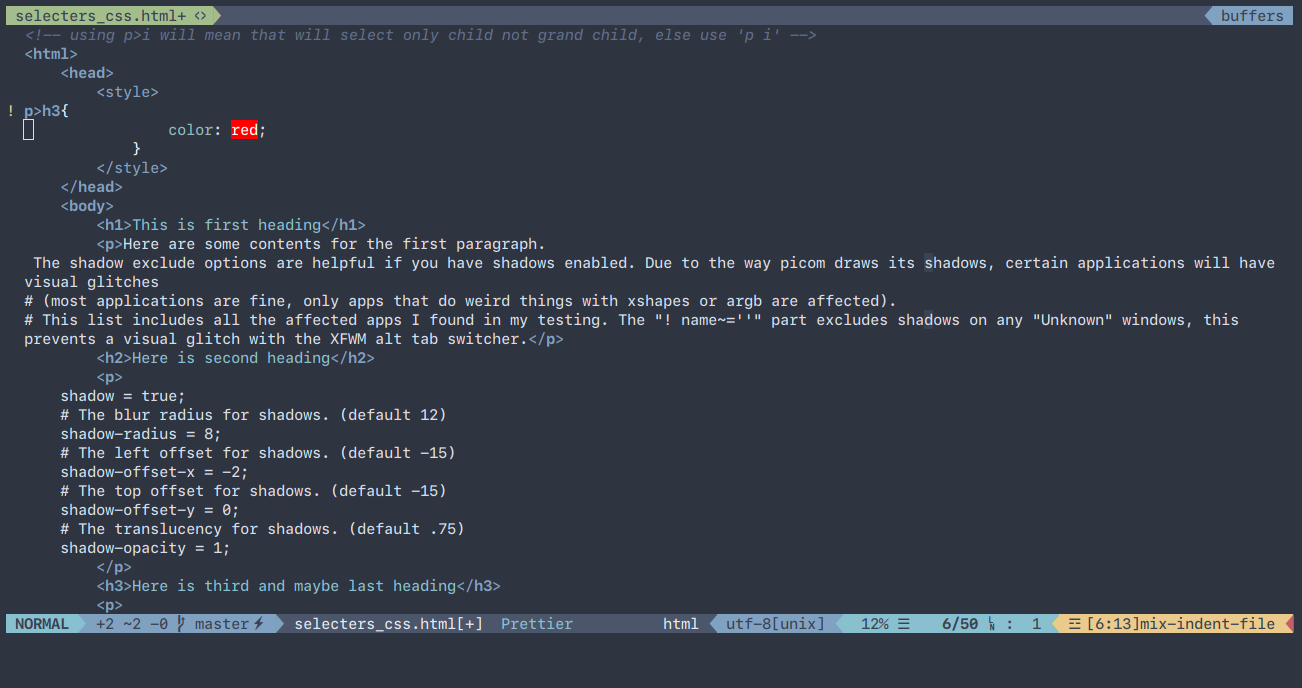
\includegraphics[width=1\textwidth]{images/2020-03-23-225605_1302x688_scrot.png}
	\caption{Child selector example}
\end{figure}

Only area of \textless p \textgreater under \textless h3 \textgreater will be highlighted.

Child selector can be combined with other selectors e.g.,
Body\textless* Selects all children of the \textless{}body\textgreater element.
Body\textless*\textless* Selects all grandchildren of the body element.
Body\textless*\textless{}p Selects all grandchildren of \textless{}body\textgreater element.

\subsubsection{Class Selector}

These selector provide a flexible way to apply style elements. Class selectors deal with the elements having that attribute class. To select elements with a specific class, write a period(.) character, followed by the name of the class.

\begin{figure}[hbt!]
	\centering
	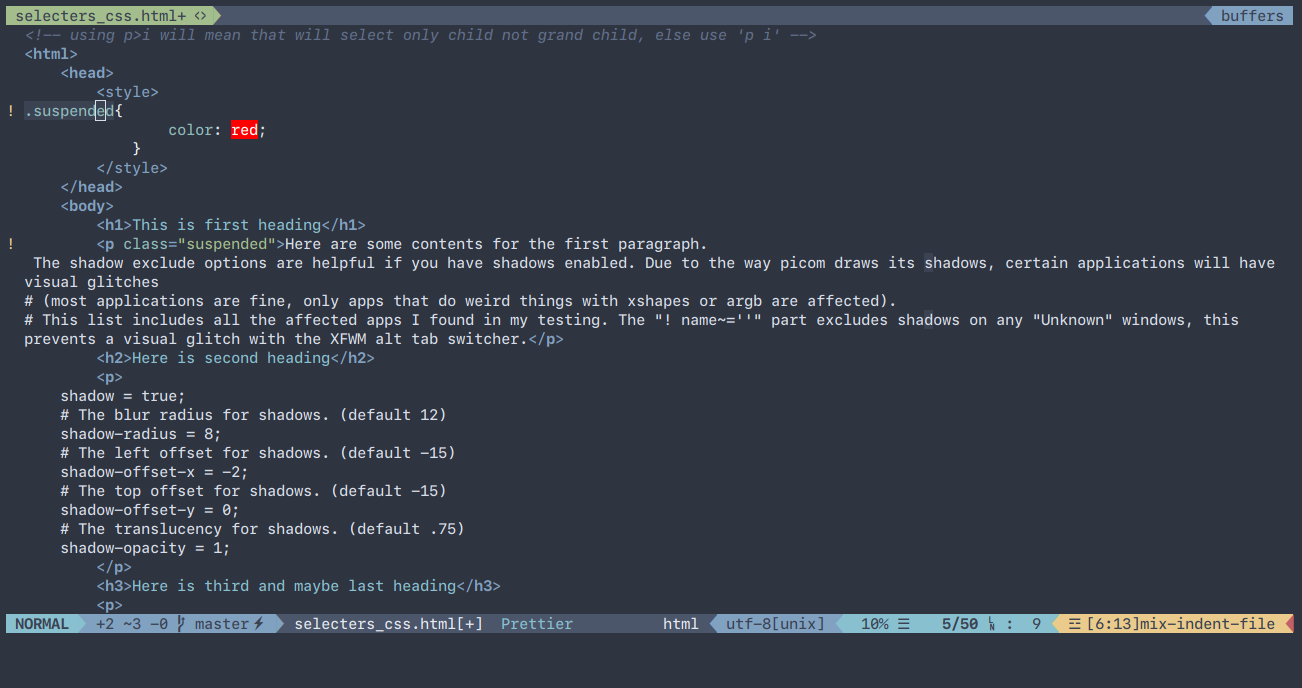
\includegraphics[width=1\textwidth]{images/2020-03-23-230041_1302x688_scrot.png}
	\caption{Screenshot showing class selector}
\end{figure}

\subsubsection{ID Selector}

The attribute id of an element is a unique indentfier in a web page. This means that no two id attribute can have the same value within the document. The id differs from class in that id identifies a single element uniquely whereas class identifies a set of an identity.

An id selector is defined by placing a \textbf{\#} symbol before selector name

\begin{figure}[hbt!]
	\centering
	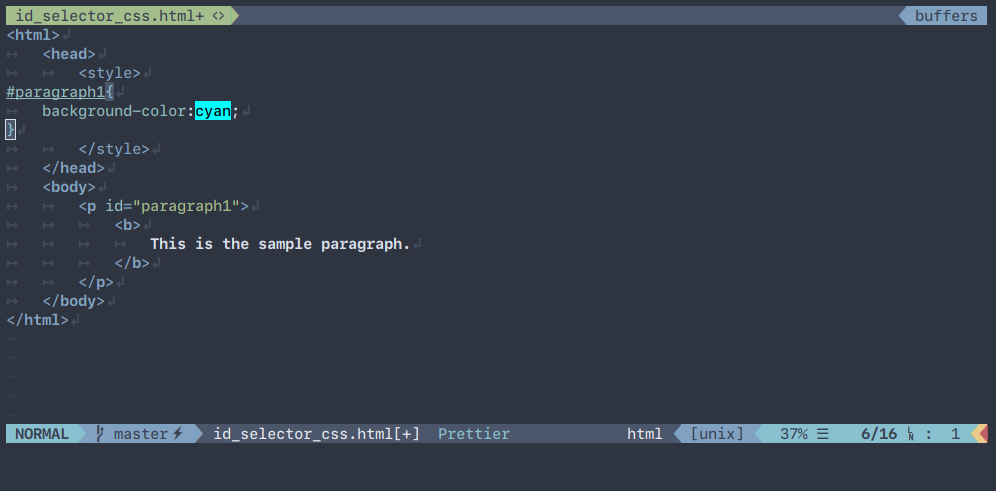
\includegraphics[width=1\textwidth]{images/2020-03-23-233023_996x491_scrot.png}
	\caption{example of ide selector}
\end{figure}

\subsubsection{Pseudo Class}

Pseudo class is a selector that selects the elements that are in specific states, e.g., They are the first element of their type or they are being handover by mouse pointer.

Pseudo classes are keywords that start with a colon

Here's an example

\begin{figure}[hbt!]
	\centering
	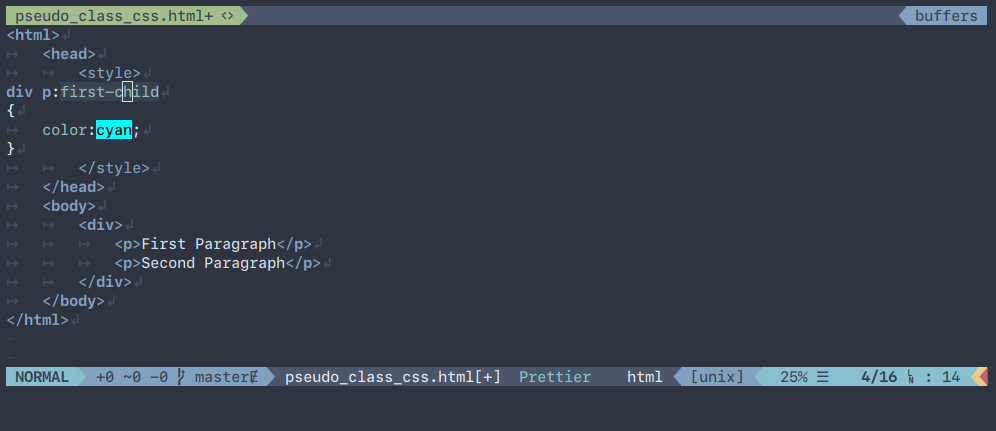
\includegraphics[width=1\textwidth]{images/2020-03-23-230626_996x431_scrot.png}
	\caption{this is how pseudo class works}
\end{figure}

\vskip 1cm

Here are few more examples of pseudo class selectors:

\begin{figure}[hbt!]
	\centering
	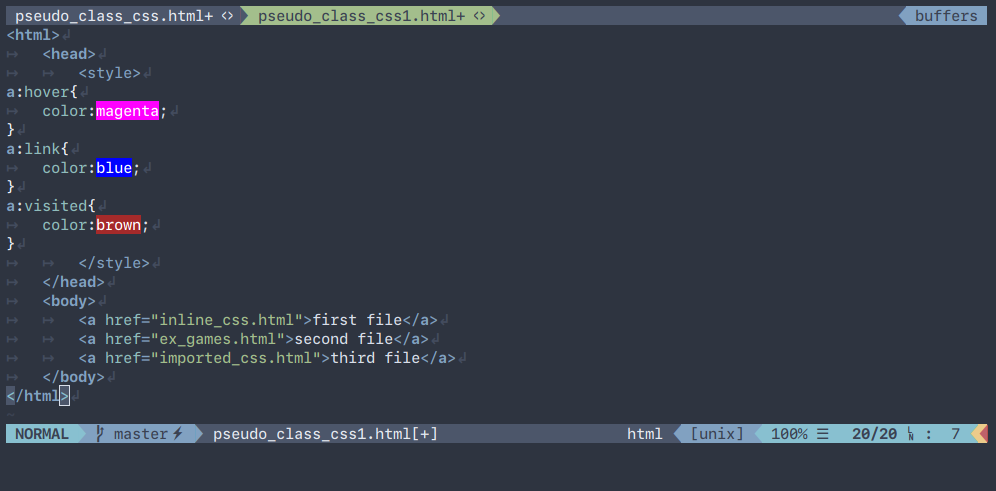
\includegraphics[width=1\textwidth]{images/2020-03-23-231213_996x491_scrot.png}
	\caption{second example of pseudo class selector}
\end{figure}

\begin{figure}[hbt!]
	\centering
	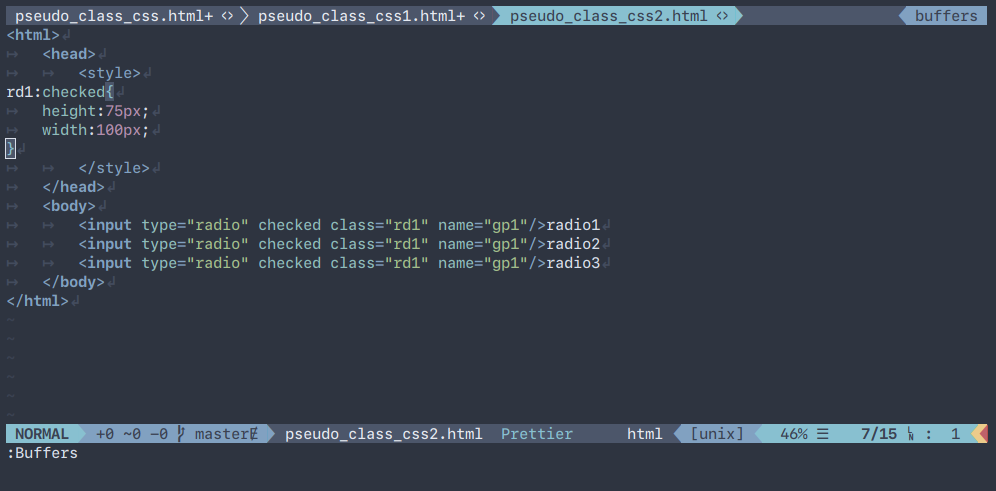
\includegraphics[width=1\textwidth]{images/2020-03-23-231849_996x491_scrot.png}
	\caption{third example of pseudo class selector}
\end{figure}

\begin{figure}[hbt!]
	\centering
	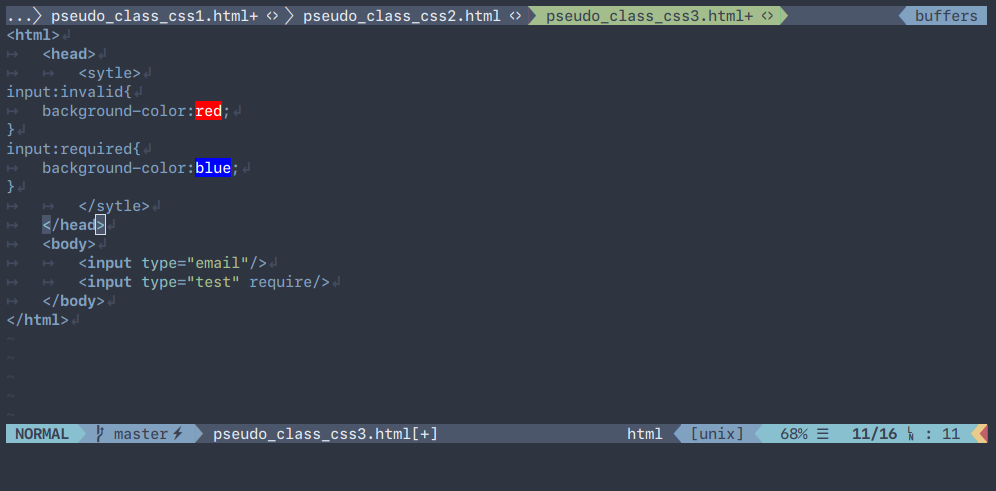
\includegraphics[width=1\textwidth]{images/2020-03-23-232050_996x491_scrot.png}
	\caption{fourth example of pseudo class selector}
\end{figure}

\subsubsection{Pseudo Element}

Pseudo element behave in similar way, however they act as if you have added a whole new html element into the markup, rather than applying a class to existing elements.

Pseudo elements start with double colon \textbf{::}

Here are few examples of pseudo element selector

\begin{figure}[hbt!]
	\centering
	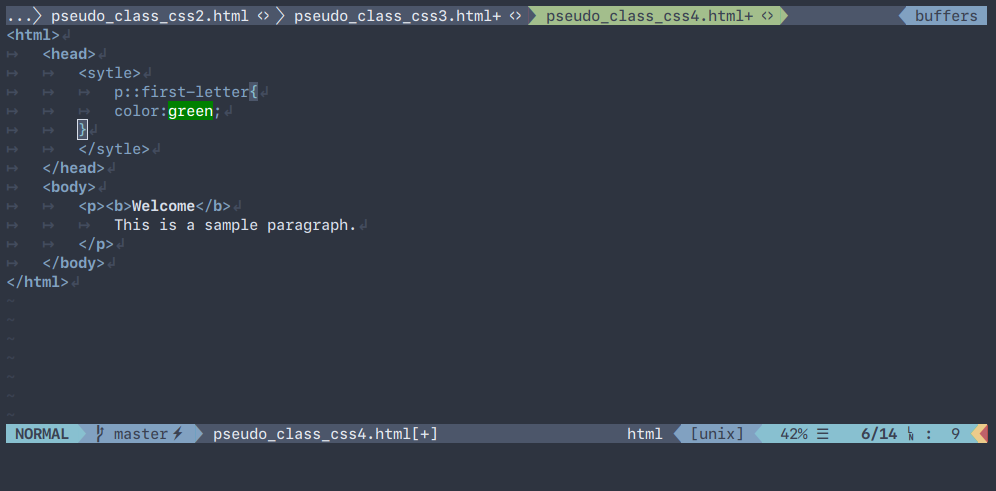
\includegraphics[width=1\textwidth]{images/2020-03-23-232348_996x491_scrot.png}
	\caption{first example of pseudo element selector}
\end{figure}

\begin{figure}[hbt!]
	\centering
	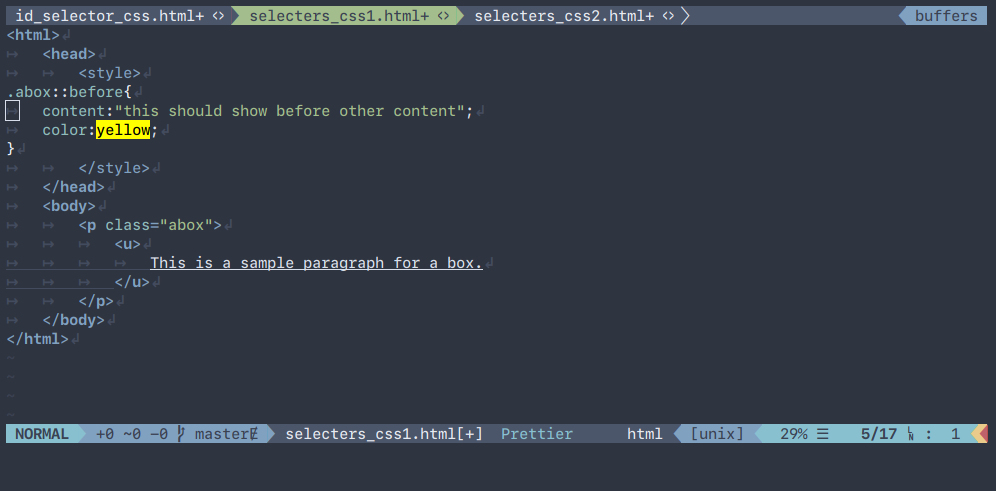
\includegraphics[width=1\textwidth]{images/2020-03-23-233647_996x491_scrot.png}
	\caption{second example of pseudo element selector}
\end{figure}

\begin{figure}[hbt!]
	\centering
	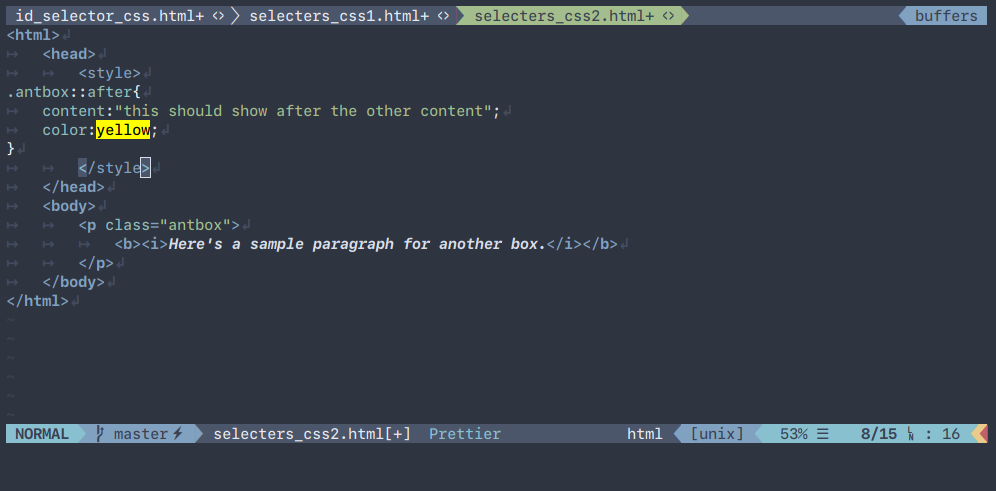
\includegraphics[width=1\textwidth]{images/2020-03-23-233736_996x491_scrot.png}
	\caption{third example of pseudo element selector}
\end{figure}

\end{document}
